\documentclass[11pt,a4paper]{article}

\usepackage[utf8]{inputenc}
\usepackage[spanish]{babel}
\usepackage{geometry}
\usepackage{graphicx}
\usepackage{booktabs}
\usepackage{tabularx}
\usepackage{amsmath}
\usepackage{xcolor}
\usepackage{hyperref}
\usepackage{fancyhdr}
\usepackage{caption}
\usepackage{float}
\usepackage{microtype}
\usepackage{listings}

\geometry{margin=2.3cm}
\graphicspath{{figuras/}}
\definecolor{azul}{HTML}{354A68}
\definecolor{lila}{HTML}{E9E4F4}
\definecolor{verde}{HTML}{E5F2EE}
\definecolor{gris}{HTML}{F5F6F8}
\hypersetup{colorlinks=true,linkcolor=azul,urlcolor=azul}
\lstset{basicstyle=\ttfamily\small,backgroundcolor=\color{gris},frame=single,
  framerule=0.3pt,breaklines=true,showstringspaces=false,columns=fullflexible}
\pagestyle{fancy}
\fancyhf{}
\fancyhead[L]{\small Desafío PIC}
\fancyhead[R]{\small Microcontroladores}
\fancyfoot[C]{\thepage}
\setlength{\headheight}{14pt}
\captionsetup{font=small,labelfont=bf}

\begin{document}

\begin{center}
  {\Large\bfseries\color{azul} Desafío PIC}\\[0.25cm]
  {\large Lectura de temperatura y luminosidad con el PIC16F877A}\\[0.45cm]
  {\normalsize Alex Díaz Canales y María José Córdova}\\[0.15cm]
  {\normalsize Ingeniería en Automatización y Robótica --- Microcontroladores}\\[0.15cm]
  {\normalsize Noviembre de 2026}
\end{center}

\noindent\colorbox{verde}{\parbox{\dimexpr\linewidth-2\fboxsep\relax}{\textbf{Estado del trabajo.}
La simulación y el programa en C funcionan. La implementación física solicitada en la pauta todavía está pendiente.}}

\section*{Antes de empezar: cómo leer este informe}

Lo escribimos pensando en alguien que conoce la idea de una variable y un \texttt{if}, pero que todavía no ha conectado un PIC. La ruta del proyecto es sencilla: una condición física cambia un voltaje; el PIC convierte ese voltaje en un número; el programa decide qué número mostrar; los displays lo dibujan con luz.

\begin{center}
\colorbox{lila}{\parbox{0.91\linewidth}{\centering
\textbf{Temperatura o luz} $\longrightarrow$ \textbf{voltaje} $\longrightarrow$
\textbf{ADC del PIC} $\longrightarrow$ \textbf{cálculo en C} $\longrightarrow$
\textbf{dos displays}}}
\end{center}

Usaremos estos nombres durante el recorrido:

\begin{center}
\small
\begin{tabularx}{\linewidth}{@{}lX@{}}
\toprule
Término & Significado en este proyecto \\
\midrule
Pin & Patita física del circuito integrado; tiene un número en el encapsulado. \\
Puerto & Grupo de pines con un nombre común, como A, B, C o D. \\
AN0 y AN1 & Canales de entrada del convertidor analógico-digital (ADC). \\
GND y VDD & Referencia de cero voltios y alimentación positiva del PIC. \\
\texttt{TRIS} y \texttt{PORT} & Registros para elegir la dirección de un pin y leer o escribir su nivel. \\
\texttt{.hex} & Archivo que contiene el programa compilado para el microcontrolador. \\
\bottomrule
\end{tabularx}
\end{center}

\section{Qué nos pidió la guía}

El desafío consiste en usar un PIC16F877A con dos entradas analógicas: un sensor de temperatura LM35 y una LDR. Un interruptor debe elegir qué sensor se presenta. Cuando se elige el LM35, la pantalla debe mostrar temperatura; cuando se elige la LDR, debe mostrar intensidad luminosa en porcentaje. La entrega considera la simulación, el código en C y el archivo \texttt{.hex}, además de un montaje físico en protoboard.

Elegimos dos displays de siete segmentos de cátodo común, una de las alternativas permitidas por la guía. Para la simulación usamos SimulIDE y para el firmware MPLAB X con XC8. En la versión de SimulIDE instalada, el componente disponible aparece como \texttt{p16F877}; el programa se compiló para el PIC16F877A. La diferencia entre el nombre del modelo simulado y el dispositivo solicitado debe quedar clara en la presentación.

\section{Diseño del circuito}

Organizamos el circuito por bloques para poder revisar cada parte por separado. La tabla resume las señales empleadas. Los números corresponden al encapsulado DIP de 40 pines del PIC16F877A, según su hoja de datos~\cite{pic}.

\begin{center}
\small
\begin{tabularx}{\linewidth}{@{}lclX@{}}
\toprule
Señal & Pin & Puerto & Función \\
\midrule
LM35 simulado & 3 & RA1/AN1 & Entrada de temperatura \\
LDR & 2 & RA0/AN0 & Entrada de luminosidad \\
Selector & 33 & RB0 & Cambia la lectura mostrada \\
Decenas & 15 & RC0 & Habilita el primer display \\
Unidades & 16 & RC1 & Habilita el segundo display \\
Segmentos $a$--$g$ & 19--22, 27--29 & RD0--RD6 & Líneas compartidas entre ambos displays \\
\bottomrule
\end{tabularx}
\end{center}

\subsection{Paso 1: alimentar, reiniciar y dar un reloj al PIC}

Todo circuito necesita un punto de referencia común. Llamamos \emph{GND} a ese cero voltios y \emph{VDD} a la alimentación positiva. En el PIC físico de 40 pines, VDD corresponde a los pines 11 y 32, y VSS (tierra) a los pines 12 y 31~\cite{pic}. El dibujo de SimulIDE muestra sus pines VDD y VSS en azul porque el modelo del microcontrolador maneja internamente la alimentación. Eso no debe copiarse literalmente a la protoboard: allí conectaremos los cuatro pines de alimentación.

El pin 1, MCLR, sirve para reiniciar el PIC. Lo mantuvimos en \(+5\,\mathrm V\) por medio de \(10\,\mathrm{k\Omega}\), y añadimos un pulsador entre MCLR y GND. Al presionarlo, MCLR pasa momentáneamente a cero. Es importante distinguir este pulsador del interruptor que selecciona el sensor: cumplen funciones distintas.

El programa supone una frecuencia de \(4\,\mathrm{MHz}\). La propiedad \emph{Frequency} del PIC en SimulIDE y la constante \texttt{\_XTAL\_FREQ} del código tienen ese mismo valor. En simulación, el reloj se genera dentro del modelo; en físico se necesitarán el cristal de 4 MHz y los condensadores de acuerdo con el circuito de reloj~\cite{simulide,pic}. Este vínculo entre frecuencia, bits de configuración y retardos aparece en las clases de las semanas 7 y 8~\cite{clasepic,claseconfig}.

\subsection{Paso 2: convertir la luz en un voltaje medible}

Una LDR es una resistencia que cambia con la luz. El PIC no mide directamente ``cantidad de luz''; su ADC mide \emph{voltaje}. Por eso conectamos una resistencia fija de \(10\,\mathrm{k\Omega}\) desde \(+5\,\mathrm V\) hasta AN0 (pin 2), y la LDR desde AN0 hasta GND. AN0 es el punto intermedio del divisor de tensión:

\begin{center}
\colorbox{gris}{\parbox{0.8\linewidth}{\centering
\(+5\,\mathrm V\) $\longrightarrow$ \(10\,\mathrm{k\Omega}\) $\longrightarrow$
\textbf{AN0} $\longrightarrow$ \textbf{LDR} $\longrightarrow$ \textbf{GND}}}
\end{center}

Cuando llega más luz, la resistencia de la LDR baja. En esta orientación también baja la tensión en AN0; el programa invierte la escala para que un valor mayor en pantalla represente más luz. La perilla que aparece bajo la LDR en SimulIDE modifica el nivel de iluminación de ese componente, no la fuente que emula al LM35.

\subsection{Paso 3: representar la salida del LM35}

Un LM35 real entrega una tensión proporcional a la temperatura: aproximadamente \(10\,\mathrm{mV}\) por cada grado Celsius~\cite{lm35}. En nuestra instalación de SimulIDE no encontramos ese componente, así que conectamos una fuente de voltaje ajustable a AN1 (pin 3). La configuramos en \(0{,}250\,\mathrm V\) para representar \(25\,{}^\circ\mathrm C\): \(250\,\mathrm{mV}/(10\,\mathrm{mV}/{}^\circ\mathrm C)=25\,{}^\circ\mathrm C\).

La fuente tiene dos indicaciones que pueden confundirse. El número \(0{,}25\,\mathrm V\) dentro del componente es el valor actual redondeado; el número rojo \(1{,}5\,\mathrm V\) debajo corresponde al límite superior configurado. Para fijar exactamente \(0{,}250\,\mathrm V\), usamos la propiedad \emph{Current Value}. Esta sustitución permite probar el programa, pero todavía no prueba el sensor físico.

\subsection{Paso 4: elegir el sensor con RB0}

El interruptor de selección está a la derecha del PIC, en RB0 (pin 33). Añadimos una resistencia de \(10\,\mathrm{k\Omega}\) desde RB0 a \(+5\,\mathrm V\); se llama \emph{pull-up} porque mantiene el pin en nivel alto cuando el interruptor está abierto. El otro extremo del interruptor va a GND. Así evitamos que la entrada quede sin un valor definido.

\begin{center}
\small
\begin{tabular}{@{}lll@{}}
\toprule
Interruptor & Nivel leído en RB0 & Dato mostrado \\
\midrule
Abierto & 1 (alto) & LDR, porcentaje relativo de luz \\
Cerrado & 0 (bajo) & LM35 simulado, temperatura \\
\bottomrule
\end{tabular}
\end{center}

La clase de MPLAB y SimulIDE emplea la misma idea de un botón con pull-up externo~\cite{clasesimulide}. En nuestra prueba, las tres fuentes fijas de \(5\,\mathrm V\) que alimentan MCLR, el divisor de la LDR y este pull-up debían estar encendidas.

\subsection{Paso 5: mostrar dos cifras con siete líneas de segmentos}

Cada display tiene siete barras llamadas $a$ a $g$. Conectamos RD0--RD6 a esas barras en ambos displays, con una resistencia de \(330\,\Omega\) por línea para limitar la corriente. Los segmentos $a$ de ambos displays comparten una señal; ocurre lo mismo con $b$, $c$ y los demás. Elegimos el puerto D porque proporciona suficientes líneas para las siete barras y dejamos RB0 libre para el selector, aunque un ejercicio anterior hubiese usado el puerto B para un solo display.

Si activáramos ambos displays al mismo tiempo, mostrarían el mismo patrón. Para distinguir decenas y unidades usamos dos transistores NPN como interruptores hacia GND. RC0 controla el cátodo común del display de decenas y RC1 el de unidades; cada base recibe la señal a través de \(1\,\mathrm{k\Omega}\). El programa enciende primero un dígito y luego el otro, repitiendo el proceso rápidamente. A esto lo llamamos \emph{multiplexación}. En SimulIDE usamos etiquetas como \texttt{SEG\_A} y \texttt{DIG\_DECENAS} para mostrar que dos puntos tienen la misma conexión sin dibujar un cable largo; en la protoboard esas etiquetas se convertirán en cables reales.

\section{Programa en MPLAB X}

\subsection{Paso 6: pasar del archivo C al \texttt{.hex}}

En MPLAB X trabajamos con un proyecto para el PIC16F877A y el compilador XC8. El archivo \texttt{sensores.c} es texto que podemos leer y modificar; el \texttt{.hex} es el resultado de compilarlo y es el archivo que carga SimulIDE en el PIC. Usamos \emph{Build Main Project} después de cambiar el código. Si el simulador ya estaba abierto, había que recargar el firmware o reiniciar la simulación para usar la versión nueva. Este recorrido de proyecto, compilación y simulación corresponde al Tutorial 2 de la clase~\cite{clasesimulide}.

El comienzo del programa declara la cabecera del dispositivo, los bits de configuración y la frecuencia de trabajo~\cite{clasepic,claseconfig}:

\begin{lstlisting}[language=C]
#include <xc.h>
#pragma config FOSC = XT
#define _XTAL_FREQ 4000000UL
\end{lstlisting}

\texttt{xc.h} permite usar nombres como \texttt{TRISA} y \texttt{ADCON1}. \texttt{FOSC = XT} selecciona el modo de oscilador previsto para el cristal, mientras que \texttt{\_XTAL\_FREQ} le informa al compilador la frecuencia necesaria para calcular \texttt{\_\_delay\_ms()} y \texttt{\_\_delay\_us()}. También desactivamos el \emph{watchdog} durante estas pruebas y activamos las opciones de arranque que aparecen en el código completo.

\subsection{Paso 7: decir qué pines son entradas y cuáles salidas}

En C, el registro \texttt{TRIS} determina la dirección: 1 significa entrada y 0 salida. El registro \texttt{PORT} permite leer una entrada o escribir el nivel de una salida~\cite{clasepic}. Aplicamos esa regla así:

\begin{lstlisting}[language=C]
TRISAbits.TRISA0 = 1; // LDR: entrada AN0
TRISAbits.TRISA1 = 1; // LM35: entrada AN1
TRISBbits.TRISB0 = 1; // interruptor selector
TRISD = 0x00;         // siete segmentos: salidas
TRISCbits.TRISC0 = 0; // decenas
TRISCbits.TRISC1 = 0; // unidades
\end{lstlisting}

El puerto A necesita además una configuración analógica. Es fácil equivocarse aquí porque en otros ejercicios de la clase se usa \texttt{ADCON1 = 0x06} para tratar esos pines como digitales. Este proyecto sí necesita el ADC: usamos \texttt{ADCON1 = 0x80}, que deja activos los canales analógicos, selecciona VDD y VSS como referencias y ordena el resultado de diez bits hacia la derecha~\cite{claseanalog}. El código no convierte a digitales los otros canales analógicos, porque no los usamos.

\subsection{Paso 8: leer una entrada analógica}

El ADC es el traductor entre voltaje y número. Con referencia de \(0\) a \(5\,\mathrm V\), un resultado de diez bits puede tomar valores entre 0 y 1023. Una tensión cercana a \(2{,}5\,\mathrm V\), por ejemplo, produce una lectura cercana a la mitad de esa escala~\cite{claseanalog}. El PIC tiene varios canales, pero el programa elige uno a la vez.

Nuestra función \texttt{leer\_adc(canal)} sigue la secuencia vista en el Tutorial 4: selecciona AN0 o AN1 en \texttt{ADCON0}, espera \(20\,\mathrm{\mu s}\) para que la entrada se estabilice, inicia la conversión, espera a que termine y une \texttt{ADRESH} con \texttt{ADRESL} para recuperar los diez bits~\cite{claseanalog}. Configuramos el reloj del ADC como \(F_{\mathrm{osc}}/8\); con \(F_{\mathrm{osc}}=4\,\mathrm{MHz}\), cada periodo del ADC dura \(2\,\mathrm{\mu s}\).

\subsection{Paso 9: transformar la lectura en temperatura o luz}

El ADC entrega un número, no grados Celsius. Como la referencia es de \(5\,\mathrm V\), la lectura 1023 representa aproximadamente \(5\,\mathrm V\). El LM35 entrega \(0{,}010\,\mathrm V\) por grado; al dividir el voltaje recuperado por esa escala, obtenemos la fórmula usada en el código:

\begin{equation}
  T\,[{}^\circ\mathrm C] \approx \frac{\mathrm{ADC}_{\mathrm{AN1}}\,500}{1023}.
\end{equation}

Por ejemplo, \(0{,}250\,\mathrm V\) equivalen aproximadamente a una lectura ADC de 51. Al sustituirla en la fórmula resulta cerca de \(25\,{}^\circ\mathrm C\). La pantalla puede cambiar un grado cerca de un límite de redondeo porque un solo paso del ADC equivale aproximadamente a \(0{,}49\,{}^\circ\mathrm C\).

Para la LDR invertimos la escala porque, con nuestro divisor, más luz produce menos voltaje en AN0:

\begin{equation}
  L\,[\%] \approx 100 - \frac{\mathrm{ADC}_{\mathrm{AN0}}\,100}{1023}.
\end{equation}

El porcentaje no es una medición calibrada en lux: depende de la LDR, del divisor y de la iluminación usada en la prueba. La operación se hace con enteros y se redondea al valor entero que cabe en los displays.

\subsection{Paso 10: decidir qué mostrar y refrescar los displays}

Dentro de \texttt{while(1)}, un \texttt{if} lee RB0: si vale 1 calcula luz desde AN0; si vale 0 calcula temperatura desde AN1. Esta es la misma lógica de decisión y repetición que practicamos al comienzo del curso~\cite{clasec}.

La función \texttt{mostrar(numero)} separa el número en decenas y unidades. Una tabla de patrones indica qué segmentos deben encenderse para cada dígito del 0 al 9. El programa apaga ambos displays, coloca el patrón de decenas en PORTD y activa RC0 durante \(5\,\mathrm{ms}\); después hace lo mismo con las unidades y RC1. Repite el ciclo mientras el PIC está encendido. El código completo y el \texttt{.hex} están en la carpeta \texttt{firmware/} de esta entrega.

\section{Pruebas en SimulIDE}

Para que otra persona pueda repetir nuestra comprobación, dejamos la secuencia que usamos con el circuito completo:

\begin{enumerate}
  \item Abrir \texttt{DesafioPIC.sim1}. El PIC tiene asignado \texttt{firmware/sensores.hex}. Al iniciar la simulación, comprobar que aparece una lectura en los dos displays. Si no aparece, cargar ese archivo desde el menú contextual del PIC.
  \item Confirmar que están activas las tres fuentes fijas de \(5\,\mathrm V\) para MCLR, el divisor LDR y el pull-up del selector. La fuente ajustable inferior corresponde solo al LM35 simulado.
  \item Cerrar el interruptor junto a RB0 y escribir \(0{,}250\,\mathrm V\) como valor actual de la fuente ajustable. La lectura que obtuvimos fue 25.
  \item Abrir ese interruptor y mover la perilla de la LDR. La cifra debe responder a la luz simulada, mientras la fuente del LM35 sigue en \(0{,}250\,\mathrm V\).
  \item Volver a cerrar el interruptor para comprobar que se presenta nuevamente la temperatura.
\end{enumerate}

Primero verificamos que el firmware cargara y que ambos displays se encendieran. Luego ajustamos la fuente que emula el LM35. Al usar la perilla, el indicador redondeaba a dos decimales y podía mostrar \(0{,}25\,\mathrm V\) mientras los displays mostraban 24. Al escribir \(0{,}250\,\mathrm V\) en la propiedad \emph{Current Value}, obtuvimos 25. Es coherente con la resolución de un ADC de diez bits con referencia de \(5\,\mathrm V\): un paso equivale aproximadamente a \(4{,}89\,\mathrm{mV}\), o \(0{,}49\,{}^\circ\mathrm C\) para esta escala del LM35.

\begin{figure}[H]
  \centering
  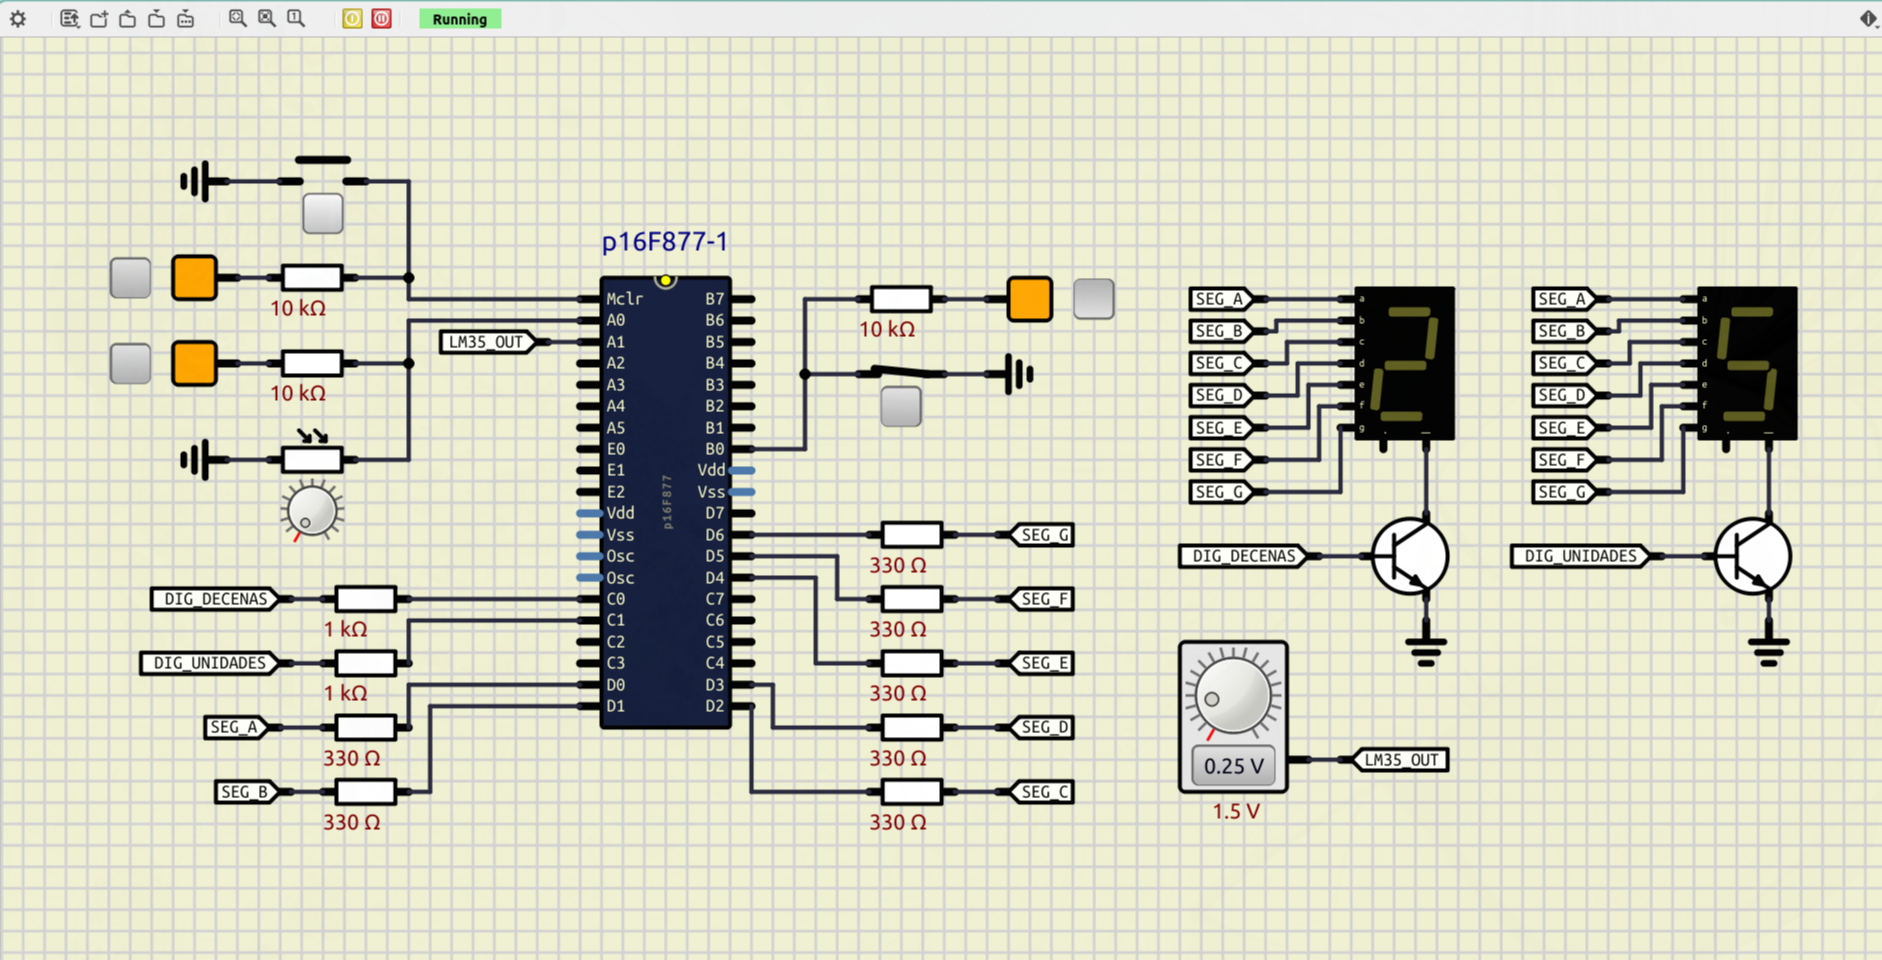
\includegraphics[width=0.70\linewidth]{temperatura_25.png}
  \caption{Simulación en modo temperatura. La fuente que representa al LM35 indica \(0{,}25\,\mathrm V\) y los displays muestran 25. Captura de nuestra prueba.}
\end{figure}

Después abrimos el selector y movimos la perilla asociada a la LDR. Las capturas de la grabación muestran dos posiciones con lecturas diferentes, 41 y 71. Estos números son salidas del circuito simulado; no los interpretamos como valores de lux ni como una calibración de la perilla.

\begin{figure}[H]
  \centering
  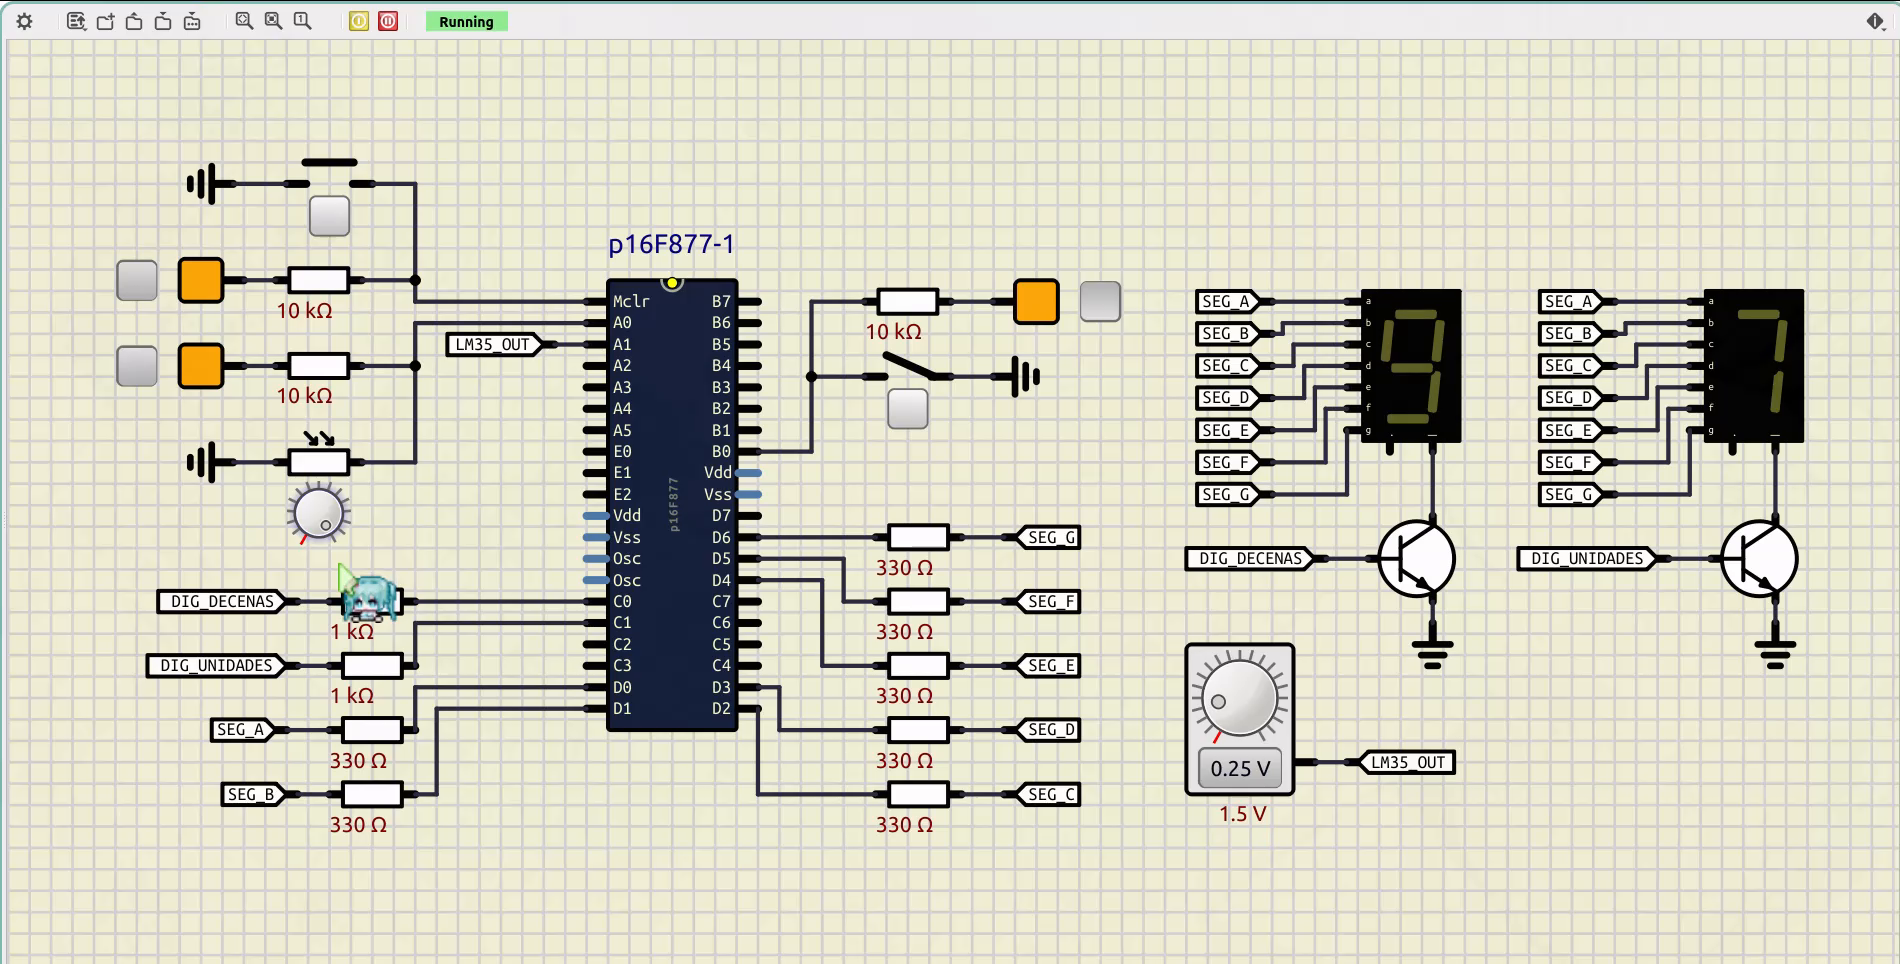
\includegraphics[width=0.70\linewidth]{luz_variacion.png}
  \caption{Una posición de la LDR en modo luz: lectura 41. Fotograma de nuestra grabación de SimulIDE.}
\end{figure}

\begin{figure}[H]
  \centering
  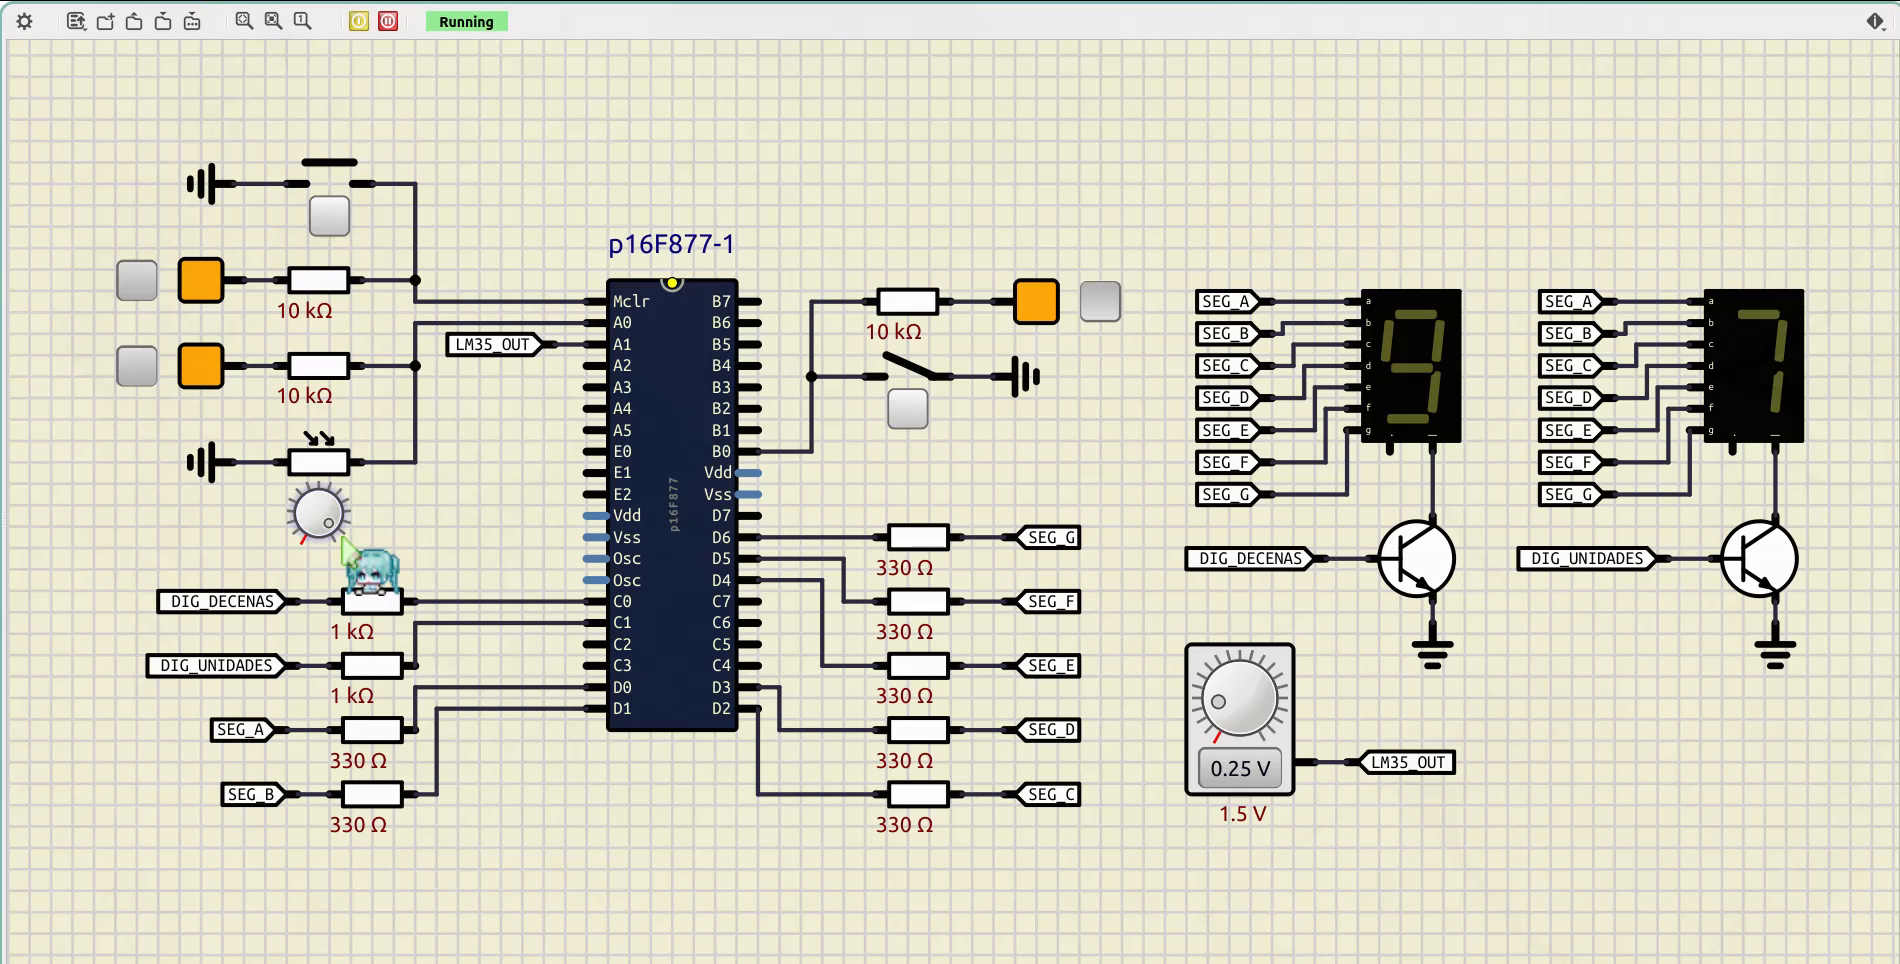
\includegraphics[width=0.70\linewidth]{luz_variacion_2.png}
  \caption{Otra posición de la LDR en modo luz: lectura 71. La fuente del LM35 permanece en \(0{,}25\,\mathrm V\).}
\end{figure}

Al guardar el circuito tuvimos que recuperar una copia anterior después de cerrar SimulIDE por accidente. Conservamos el cableado y restauramos el estado de las fuentes. Finalmente dejamos un archivo \texttt{DesafioPIC.sim1} con una ruta relativa al \texttt{.hex} y la recarga al iniciar la simulación. La captura más reciente confirma que esa copia vuelve a mostrar 25 al arrancar.

\section{Qué falta y qué aprendimos}

La simulación demuestra la selección de entradas, la conversión ADC y la visualización multiplexada. Todavía no demuestra el comportamiento de un LM35 real ni completa el montaje físico exigido por la pauta. Antes de llevarlo a protoboard tendremos que revisar el pinout exacto de los displays y transistores adquiridos, además de instalar la alimentación, el reloj y los condensadores de desacoplo del PIC.

También encontramos un límite de presentación: dos dígitos solo permiten mostrar de 00 a 99. El firmware limita a 99 cualquier valor calculado superior, incluido el extremo de 100\,\% de luz. En la demostración debemos explicar esta decisión o cambiar el sistema de visualización si se exige representar 100 de forma literal.

Este trabajo nos sirvió para separar fallas de cableado, configuración del ADC y presentación. La comparación entre el esquema de la guía, los pines del PIC y el comportamiento de SimulIDE fue importante, sobre todo al conectar los transistores y al interpretar la lectura de la fuente ajustable.

\section*{Archivos entregados}

\begin{itemize}
  \item \texttt{DesafioPIC.sim1}: circuito principal de SimulIDE.
  \item \texttt{firmware/sensores.c}: programa en C para MPLAB X y XC8.
  \item \texttt{firmware/sensores.hex}: firmware compilado.
  \item \texttt{informe/informe\_desafiopic.tex} y su PDF: informe y capturas de pantalla.
\end{itemize}

\newpage
\section*{Si alguien quiere repetir la práctica}

La relación con las clases se puede seguir en cuatro ideas: el \texttt{if} decide entre las dos entradas; \texttt{while(1)} mantiene el programa funcionando; \texttt{TRIS} define qué pines reciben o envían señales; y \texttt{ADCON0}/\texttt{ADCON1} permiten transformar voltajes en números. El display es la salida visible de esa cadena. Si un resultado no coincide con lo esperado, conviene revisar la cadena desde la entrada hasta la salida, en este orden:

\begin{center}
\small
\begin{tabularx}{\linewidth}{@{}lX@{}}
\toprule
Lo que se observa & Primera comprobación \\
\midrule
Displays apagados & Confirmar que SimulIDE está ejecutándose, que las fuentes de \(5\,\mathrm V\) están activas y que el PIC cargó \texttt{sensores.hex}. \\
Marca 24 con ``0,25 V'' & Abrir las propiedades de la fuente y escribir \(0{,}250\,\mathrm V\) en \emph{Current Value}; la perilla y el indicador pueden redondear. \\
La LDR no altera la cifra & Abrir el interruptor de RB0; luego comprobar el divisor entre \(+5\,\mathrm V\), AN0, la LDR y GND. \\
No cambia entre modos & Revisar el pull-up de RB0 y el cable entre el interruptor y GND. \\
Un dígito no enciende & Revisar su transistor, la resistencia de base y la señal RC0 o RC1 correspondiente. \\
\bottomrule
\end{tabularx}
\end{center}

Estas comprobaciones describen la simulación. En el montaje físico añadiremos la verificación de voltajes reales y del pinout del componente que tengamos en la mano.

\begin{thebibliography}{9}
\bibitem{pic} Microchip Technology, \emph{PIC16F87XA Data Sheet}, DS39582B. \url{https://ww1.microchip.com/downloads/en/DeviceDoc/39582b.pdf}.
\bibitem{lm35} Texas Instruments, \emph{LM35 Precision Centigrade Temperature Sensors}, hoja de datos. \url{https://www.ti.com/lit/ds/symlink/lm35.pdf}.
\bibitem{simulide} SimulIDE, \emph{MCUs: Basic Use and Properties}. \url{https://simulide.com/p/mcus/}.
\bibitem{clasec} Material de clase de Microcontroladores, \emph{Semana 1: Lenguaje C} y \emph{Semana 2: if, else y while}, 2026.
\bibitem{clasepic} Ángel Custodio, \emph{Tutorial 1: Programación del PIC16F877A en C}, material de Microcontroladores, semana 7, 2026.
\bibitem{clasesimulide} Ángel Custodio, \emph{Tutorial 2: Del código a la simulación: MPLAB X, Proteus y SimulIDE}, material de Microcontroladores, semana 7, 2026.
\bibitem{claseconfig} Ángel Custodio, \emph{Tutorial 3: Bits de configuración del PIC16F877A}, material de Microcontroladores, semana 8, 2026.
\bibitem{claseanalog} Ángel Custodio, \emph{Tutorial 4: Convertidor ADC del PIC16F877A}, material de Microcontroladores, semana 9, 2026.
\bibitem{guia} Guía del \emph{Desafío PIC} entregada en la asignatura Microcontroladores, imágenes de la pauta y circuitos sugeridos proporcionadas por el docente.
\end{thebibliography}

\end{document}
